\documentclass[sigconf]{acmart}
\usepackage{tikz}
\usetikzlibrary{positioning,calc}
\usetikzlibrary{decorations.text}
\usetikzlibrary{decorations.pathmorphing,decorations.pathreplacing}
\usetikzlibrary{arrows,petri, topaths,fit}
\usepackage{tcolorbox}

\begin{document}

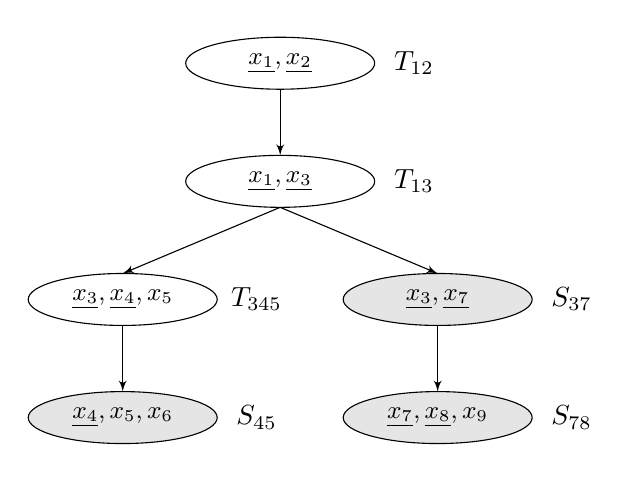
\begin{tikzpicture}
			\tikzset{edge/.style = {->,> = latex'},
				vertex/.style={circle, thick, minimum size=5mm}}
			\def\x{0.25}
			
			\begin{scope}[fill opacity=1]
			
			\draw[] (0,-2) ellipse (1.2cm and 0.33cm) node {\small \small ${\underline{x_1}, \underline{x_2}}$};
			\node[vertex]  at (1.7,-2) {$T_{12}$};
			\draw[] (0,-3.5) ellipse (1.2cm and 0.33cm) node {\small \small ${\underline{x_1}, \underline{x_3}}$};
			\node[vertex]  at (1.7,-3.5) {$T_{13}$};				
			\draw[] (-2,-5) ellipse (1.2cm and 0.33cm) node {\small \small ${\underline{x_3}, \underline{x_4}, x_5}$};		
			\node[vertex]  at  ( -0.3,-5) {$T_{345}$};	
			
			\draw[fill=black!10] ( 2,-5) ellipse (1.2cm and 0.33cm) node {\small \small ${\underline{x_3}, \underline{x_7}}$};		
			\node[vertex]  at  ( 3.7,-5) {$S_{37}$};	
            
            \draw[fill=black!10] ( -2,-6.5) ellipse (1.2cm and 0.33cm) node {\small \small ${\underline{x_4}, x_5, x_6}$};	\node[vertex]  at  ( -0.3, -6.5) {$S_{45}$};	
            
            \draw[fill=black!10] ( 2,-6.5) ellipse (1.2cm and 0.33cm) node {\small \small ${\underline{x_7}, \underline{x_8}, x_9}$};	\node[vertex]  at  ( 3.7, -6.5) {$S_{78}$};	
            
			\draw[edge] (0,-2.33) -- (0,-3.17);	
			\draw[edge] (0,-3.83) -- (-2,-4.67);	
			\draw[edge] (0,-3.83) -- ( 2,-4.67);
			\draw[edge] (-2, -5.33) -- ( -2, -6.17);
			
			\draw[edge] ( 2, -5.33) -- ( 2, -6.17);
			
			\end{scope}	
			\end{tikzpicture}

\end{document}